\documentclass{beamer}
\usepackage{pgf,tikz}
\usetikzlibrary{positioning, decorations.markings}

\newcommand{\isomorphism}{\simeq}
\newtheorem{proposition}{Proposition}

\title{Graph Theory}
\author{Module 1}
\institute{Section 5 : Paths and Connectedness}

\begin{document}
\begin{frame}
	\maketitle
\end{frame}

\begin{frame}
\frametitle{Walk}
\begin{definition}[walk]
	A walk is an alternating finite sequence $W : v_0e_1v_1e_2v_2\dots e_pv_p$ where $v_{j-1}$ and $v_j$ are end vertices of $e_j$ for $j = 1,2,\dots$.
\end{definition}
The length of a walk is the number of edges in it.
\begin{description}
	\item[origin] is the vertex $v_0$.
	\item[terminus] is the vertex $v_p$,
	\item[closed] A walk is closed if $v_0 = v_p$.
	\item[trail] is a walk in which every edges are distinct.
	\item[path] is a walk in which every vertex is distinct.
	\item[cycle] is a closed trail.
\end{description}
\end{frame}

\begin{frame}
\frametitle{Path}
\begin{description}
	\item[$C_k$] is a cycle of length $k$.
	\item[$P_k$] is a path on $k$ vertices.
	\item[Path, $P$] Let $P : v_1,e_1,v_2,\dots,e_p,v_p$ be a path in $G$. Then we omit edges and write $P : v_1,v_2,\dots,v_p$.
	\item[Inverse of $P$] The path $P' : v_p,v_{p-1},\dots,v_1$ is the inverse of $P$.
	\item[section of $P$] Let $P : v_1,v_2,\dots,v_p$ be a path in $G$.
	A subsequence $v_j,v_{j+1},\dots,v_k$ is $v_j-v_k$ section of $P$.
\end{description}
\end{frame}

\begin{frame}
\frametitle{Connected}
\begin{definition}
	Two vertices $u,v$ are connected in a graph $G$ if there is a $u-v$ path in $G$.
\end{definition}
\begin{definition}
	A graph $G$ is connected if every pair of vertices in $G$ are connected.
\end{definition}
\end{frame}

\begin{frame}
	\frametitle{Equivalence Relation : Connectedness}
\begin{description}
	\item[reflexive] Every vertex is connected to itself by trivial path.
	\item[symmetric] every $u-v$ path is a $v-u$ path
	\item[transitive] $u-v$ path followed by $v-w$ path contains a $u-w$ path.
\end{description}

\begin{definition}[component]
	Let $V_1,V_2,\dots,V_\omega$ be the equivalence classes of the relation `connectedness' in $G$.
	Then the induced subgraphs $G[V_1], G[V_2],\dots, G[V_\omega]$ are the component of $G$.
\end{definition}
\begin{itemize}
	\item If $\omega = 1$, then $G$ is connected.
	\item If $\omega \ge 2$, then $G$ is disconnected.
\end{itemize}
\end{frame}

\begin{frame}
\frametitle{Metric Space}%1.5.5
\begin{definition}
	Let $d$ be a function on the vertex set of a graph $G$ defined as $d(u,v)$ is the length of the shortest $u-v$ path in $G$.
\end{definition}

\begin{block}{Function $d$ is a metric on $V(G)$}
\begin{enumerate}
	\item $d(u,v) \ge 0$ and $d(u,v) = 0 \iff u = v$.
	\item $d(u,v) = d(v,u)$
	\item $d(u,v) \le d(u,w) + d(w,v)$.
\end{enumerate}
\end{block}
\end{frame}

\begin{frame}
	\frametitle{Minimum Degree of a Simple, Connected Graph}%1.5.6
	\begin{proposition}
		If $G$ is simple and $\delta(G) \ge \frac{n-1}{2}$, then $G$ is connected.
	\end{proposition}
	\begin{proof}
	\begin{itemize}
		\item Let $G$ be disconnected graph of order $n$.
		\item Suppose $G$ has at least two components.
		\item Number of vertices in each component is at least $\frac{n-1}{2}+1$.
		\item Number of vertices in $G$ is $n+1$.(contradiction)
	\end{itemize}
	\end{proof}
\end{frame}

\begin{frame}
\frametitle{Exercises : Minimum Degree}
\begin{itemize}
	\item There exists non-simple disconnected graph $G$ with $\delta(G) \ge (n-1)/2$.
	\begin{itemize}
		\item Draw a graph with two components.
		\item Use parallel edge or loops to increase minimum degree of the graph.
	\end{itemize}
	\item $\delta(G) \ge (n-2)/2$ does not imply that $G$ is connected.
	\begin{itemize}
		\item If $\delta(G) = 1$, then we have a graph of order $4$, say $2K_2$
		\item In general, $2K_{\delta(G)+1}$ has order $n = 2\delta(G) + 2$.
	\end{itemize}
\end{itemize}
\end{frame}

\begin{frame}
\frametitle{Ramsey Number, $R(3,3) = 6$}
	In a group of six people, there must be three people who are mutually acquainted or three people are not mutually acquainted.
\begin{itemize}
	\item Let $u \in V(G)$. Then $deg(u) \ne 0$ 
	\item $\Delta(G) \ne 1$. 
	\item Let $deg(u) = 2$. Let $uv,uw \in E(G)$.
	\item $vw \notin E(G)$ otherwise $(u,v,w)$ forms $\triangle$.
	\item WLOG $vx \in E(G)$, otherwise $(v,w,x)$ forms $\triangle$.
	\item $ux \notin E(G)$, otherwise $(u,v,x)$ forms $\triangle$.
	\item Similarly, $uy,uz \notin E(G)$.
	\item $xy \in E(G)$, otherwise $(u,x,y)$ forms $\triangle$.
	\item Similarly, $yz,zx \in E(G)$.
	\item \alert{$(x,y,z)$ forms $\triangle$ (contradiction)}
\end{itemize}
\begin{figure}
\centering
\scalebox{0.8}{
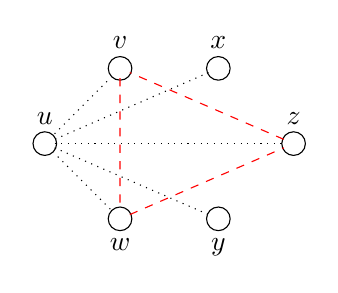
\begin{tikzpicture}
	\draw node (u)[label=above:$u$]{};
	\draw node (v)[above right=1cm of u,label=above:$v$]{};
	\draw node (w)[below right=1cm of u,label=below:$w$]{};
	\draw node (x)[right=1cm of v,label=above:$x$]{};
	\draw node (y)[right=1cm of w,label=below:$y$]{};
	\draw node (z)[below right=1cm of x,label=above:$z$]{};
	\draw (u) circle (0.15cm);
	\draw (v) circle (0.15cm);
	\draw (w) circle (0.15cm);
	\draw (x) circle (0.15cm);
	\draw (y) circle (0.15cm);
	\draw (z) circle (0.15cm);
	\draw[dotted] (w)--(u)--(v);
	\draw[dotted] (x)--(u)--(y);
	\draw[dotted] (u)--(z);
	\draw[dashed,red] (v)--(w)--(z)--(v);
\end{tikzpicture}

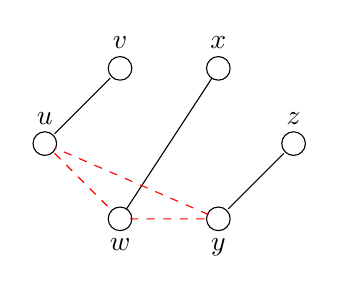
\begin{tikzpicture}
	\draw node (u)[label=above:$u$]{};
	\draw node (v)[above right=1cm of u,label=above:$v$]{};
	\draw node (w)[below right=1cm of u,label=below:$w$]{};
	\draw node (x)[right=1cm of v,label=above:$x$]{};
	\draw node (y)[right=1cm of w,label=below:$y$]{};
	\draw node (z)[below right=1cm of x,label=above:$z$]{};
	\draw (u) circle (0.15cm);
	\draw (v) circle (0.15cm);
	\draw (w) circle (0.15cm);
	\draw (x) circle (0.15cm);
	\draw (y) circle (0.15cm);
	\draw (z) circle (0.15cm);
	\draw (u)--(v);
	\draw (w)--(x);
	\draw (y)--(z);
	\draw[dashed,red] (u)--(w)--(y)--(u);
\end{tikzpicture}

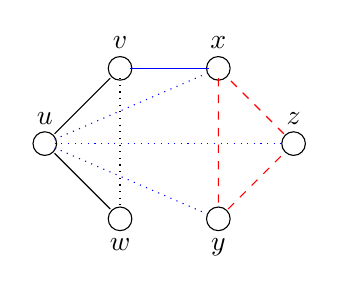
\begin{tikzpicture}
	\draw node (u)[label=above:$u$]{};
	\draw node (v)[above right=1cm of u,label=above:$v$]{};
	\draw node (w)[below right=1cm of u,label=below:$w$]{};
	\draw node (x)[right=1cm of v,label=above:$x$]{};
	\draw node (y)[right=1cm of w,label=below:$y$]{};
	\draw node (z)[below right=1cm of x,label=above:$z$]{};
	\draw (u) circle (0.15cm);
	\draw (v) circle (0.15cm);
	\draw (w) circle (0.15cm);
	\draw (x) circle (0.15cm);
	\draw (y) circle (0.15cm);
	\draw (z) circle (0.15cm);
	\draw (v)--(u)--(w);
	\draw[dotted] (v)--(w);
	\draw[blue] (v)--(x);
	\draw[dotted,blue] (u)--(x);
	\draw[dotted,blue] (u)--(y);
	\draw[dotted,blue] (u)--(z);
	\draw[dashed,red] (x)--(y)--(z)--(x);
\end{tikzpicture}
}
\end{figure}
\end{frame}

\begin{frame}
\frametitle{Complement of a disconnected Graph} %1.5.7
\begin{theorem}
	If a simple graph $G$ is disconnected, then $G^c$ is connected.
\end{theorem}
\begin{proof}
\begin{itemize}
	\item Let $G$ be a disconnected graph. 
	\item Let $G_1$ and $G_2$ be two components of $G$.
	\begin{itemize}
		\item Let $u \in V(G_1)$ and $v \in V(G_2)$.\\
		$uv \notin G \implies uv \in G^c$.
	\item Let $u,w \in V(G_1)$ and $v \in V(G_2)$.\\
		$uv,vw \notin G \implies u,v,w$ is a $u-w$ path in $G^c$.
	\end{itemize}
\end{itemize}
\end{proof}
\end{frame}

\begin{frame}
\frametitle{Characterisation of Self complementary Graph}
If $G$ is self complementary, then $n(G) \cong 0 \text{ or } 1 \pmod{4}$.
\begin{itemize}
	\item $m(G) = m(G^c) = m(K_n)/2$.
	\item $m = n(n-1)/4$.
	\item $m \cong 0 \text{ or } 1 \pmod{4}$.
\end{itemize}
\vfill
A self complementary graph with one pendant vertex must have at least another pendant vertex.
\begin{itemize}
	\item Let $G$ be a self complementary graph with pendant vertex $u$.
	\item $G^c$ has a pendant vertex $v$.
	\item $v$ is another pendant vertex in $G$.
\end{itemize}
\end{frame}

\begin{frame}
\frametitle{Upper bound for the size of a Simple Graph}%1.5.8
\begin{theorem}
	The size $m$ of simple graph of order $n$ with $\omega$ components cannot exceed $(n-\omega)(n-\omega+1)/2$.
\end{theorem}
	$$ m < \frac{(n-\omega)(n-\omega+1)}{2}$$
\begin{proof}
\begin{itemize}
	\item Let $G$ be a graph of order $n$, size $m$, and components $\omega$.
	\item Let $G_1,G_2,\dots,G_\omega$ be the components of $G$.
	\item Let $n_i,m_i$ be the order, size of $G_i$ for each $i$.
	\begin{itemize}
		\item $n_i \le (n-\omega+1)$.
		\item $m_i \le n_i(n_i-1)/2$.
	\end{itemize}
	\item $m = \sum n_i(n_i-1)/2 < (n-\omega+1) \sum (n_i - 1)$.
	\item $m < (n-\omega+1)(n-\omega)/2$.
\end{itemize}
\end{proof}
\end{frame}

\begin{frame}
\frametitle{Local Connectedness}%1.5.9
\begin{definition}
	A graph $G$ is locally connected if for each vertex $v$ in $G$, the subgraph induced by the open neighbhourhood $N_G(v)$ is connected.
\end{definition}

\begin{figure}
\centering
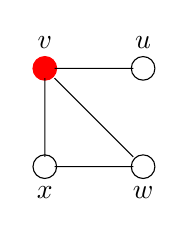
\begin{tikzpicture}
	\draw node (u)[label=above:$u$]{};
	\draw (u) circle (0.15cm);
	\draw node (v)[left=1cm of u,label=above:$v$]{};
	\draw[fill,red] (v) circle (0.15cm);
	\draw node (w)[below=1cm of u,label=below:$w$]{};
	\draw (w) circle (0.15cm);
	\draw node (x)[left=1cm of w,label=below:$x$]{};
	\draw (x) circle (0.15cm);
	\draw (u) -- (v) -- (x) -- (w) -- (v);
\end{tikzpicture}
\hspace{2cm}
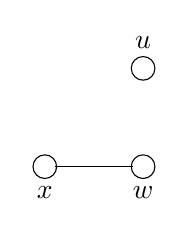
\begin{tikzpicture}
	\draw node (u)[label=above:$u$]{};
	\draw (u) circle (0.15cm);
	\draw node (w)[below=1cm of u,label=below:$w$]{};
	\draw (w) circle (0.15cm);
	\draw node (x)[left=1cm of w,label=below:$x$]{};
	\draw (x) circle (0.15cm);
	\draw (x) -- (w);
\end{tikzpicture}
	\caption{$G$ is locally connected at $x$, $u$ and $w$, but not at $v$}
\end{figure}

\end{frame}

\begin{frame}
\frametitle{Characterisation of Bipartite Graph}%1.5.10
\begin{theorem}
	A graph is bipartite if and only if it has no odd cycles.
\end{theorem}
\begin{proof}
\begin{itemize}
	\item Suppose $G$ is bipartite.
	\begin{itemize}
		\item Let $u \in V(G)$.
		\item Let $C : v_1,e_1,v_2,\dots,v_k,e_k,e_1$ be a cycle in $G$.
		\item Length of cycle $k$ is even, since $v_k$ adjacent to $v_1$.
	\end{itemize}
	\item Suppose $G$ has no odd cycle.
	\begin{itemize}
		\item Suppose $G$ is connected.
		\item \alert{$X = \{ v \in V(G) : d(u,v) \text{ is even.}\}$}
		\item \alert{$Y = \{ v \in V(G) : d(u,v) \text{ is odd.} \}$}
		\item Let $v,w \in X$. Then $u-v$ path $P$ and $u-w$ path $Q$.
		\item Let $w_1$ be a common vertex $P,Q$ such that $w_1-w$ section of $P$ and $w_1-v$ section of $Q$ has no other common vertices.
		\item Suppose $v$ is adjacent to $w$.
		\item $w-w_1 + w_1-v + vw$ is an odd cycle.(contradiction)
		\item If $G$ has components. Then $X = \cup X_i$ and $Y = \cup Y_i$.
	\end{itemize}
\end{itemize}
\end{proof}
\end{frame}

\begin{frame}
\frametitle{}
	A simple nontirivial graph $G$ is connected if and only if for any partition $(V_1,V_2)$ of $V(G)$ there is an edge joining a vertex of $V_1$ and a vertex of $V_2$.
\begin{itemize}
	\item Suppose $G$ is connected.
	\begin{itemize}
		\item Let $V_1,V_2$ be a partition of $V(G)$.
		\item Let $u \in V_1$ and $v \in V_2$.
		\item Since $G$ is connected, there exists $u-v$ path, say $P$.
		\item $P$ contains an edge joining $V_1$ and $V_2$.
	\end{itemize}
	\item Suppose that for every partition $(V_1,V_2)$, there exists an edge joining $V_1$ and $V_2$.
	\begin{itemize}
		\item Let $u,v \in V(G)$.
		\item Let $V_1 = \{ u \}$. There exists $uw \in E(G)$ where $w \in V_2$.
		\item Let $V_1 = \{ u,w \}$. There exists $ux$ or $wx$ where $x \in V_2$.
		\item Continuing like this, we get $V_1$ containing both $u$ and $v$.
	\end{itemize}
\end{itemize}
\end{frame}

\begin{frame}
\frametitle{Longest paths does intersect}
	In a connected graph $G$ with at least three vertices, any two longest paths have a vertex in common.
\begin{itemize}
	\item Let $u_1-u_k$ and $v_1-v_k$ be two longest paths, say $P,Q$.
	\item $u_1-v_1$ path has three sections : $u_1-u_r, u_r-v_s,v_s-v_1$.
	\item WLOG suppose $u_1-u_r$ and $v_1-v_s$ are at least half as long as longest paths.
	\item \alert{Then $(u_1-u_r) + (u_r-v_s) + (v_s-v_1)$ is longer. (contradiction)}
\end{itemize}
\end{frame}

\begin{frame}
\frametitle{Union of Disjoint Paths}
	Union of two disjoint paths joining two distinct vertices contains a cycle.
\begin{itemize}
	\item Let $P,Q$ be two distinct $u-v$ paths.
	\item Let $P', Q'$ be disjoint sections of $P,Q$ with common end vertices.
	\item $P'+Q'$ is a cycle.
\end{itemize}
	Union of two distinct walks joining two distinct vertices need not contain a cycle.
\begin{itemize}
	\item Two walks are distinct if one walk visits an edge one more time compared to the other.
\end{itemize}
\end{frame}

\begin{frame}
\frametitle{Characterisation of an incomplete Graph}
		If a simple graph $G$ is not complete, there exists three vertices $u,v,w$ such that $uv,vw$ are edge of $G$ but $uw$ is not an edge of $G$.
\end{frame}

\begin{frame}
\frametitle{Generalised Petersen Graph}
	\begin{definition}[Generalised Petersen Graph]
	Generalised Petersen Graph is defined by
		$$ V(P(n,k)) = \{ a_i,b_i : 0 \le i \le n-1 \}  $$
		$$ E(P(n,k)) = \{ a_ia_{i+1}, a_ib_i, b_ib_{i+k}, 0 \le i \le n-1 \} $$
	\end{definition}
	
		If $n$ is even and $k$ is odd, then generalised Petersen Graph $P(n,k)$ is bipartite.
\end{frame}

\begin{frame}
		If $G$ is simple and $\delta(G) \ge k$, then $G$ contains a path of length at least $k$.
\begin{itemize}
	\item Each component of $G$ has at least $k+1$ vertices.
	\item Apply finite mathematical induction on $\delta(G)$.
	\begin{itemize}
		\item $k =1$ is trivial
		\item Suppose graph of $\delta(G) = k-1$ has a path of length $k-1$.
		\item Suppose $\delta(G) = k$.
		\item Additional vertex which is  adjacent to one of the end vertices.
	\end{itemize}
\end{itemize}
\end{frame}

\begin{frame}
	\vspace{0.6in}
	\hspace{3cm} {\color{blue}\Huge{Thank You}}
\end{frame}
\end{document}
